

\section{System Architecture}\label{sec:architecture}

\begin{figure*}[t]
    \centering
    \begin{subfigure}[t]{0.8\textwidth}
%        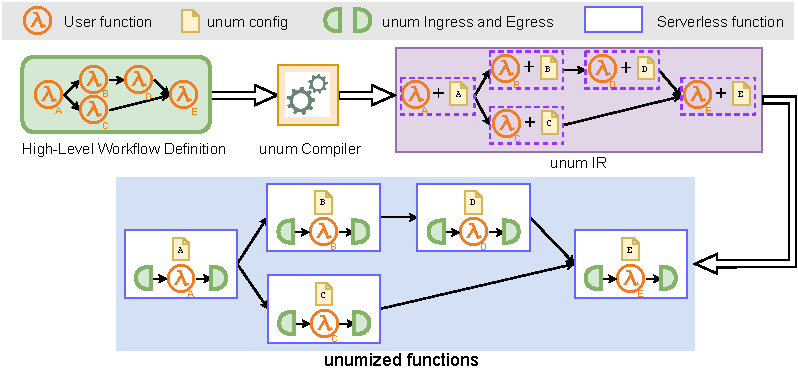
\includegraphics[width=\columnwidth]{figures/unum-arch-compile-time.pdf}
   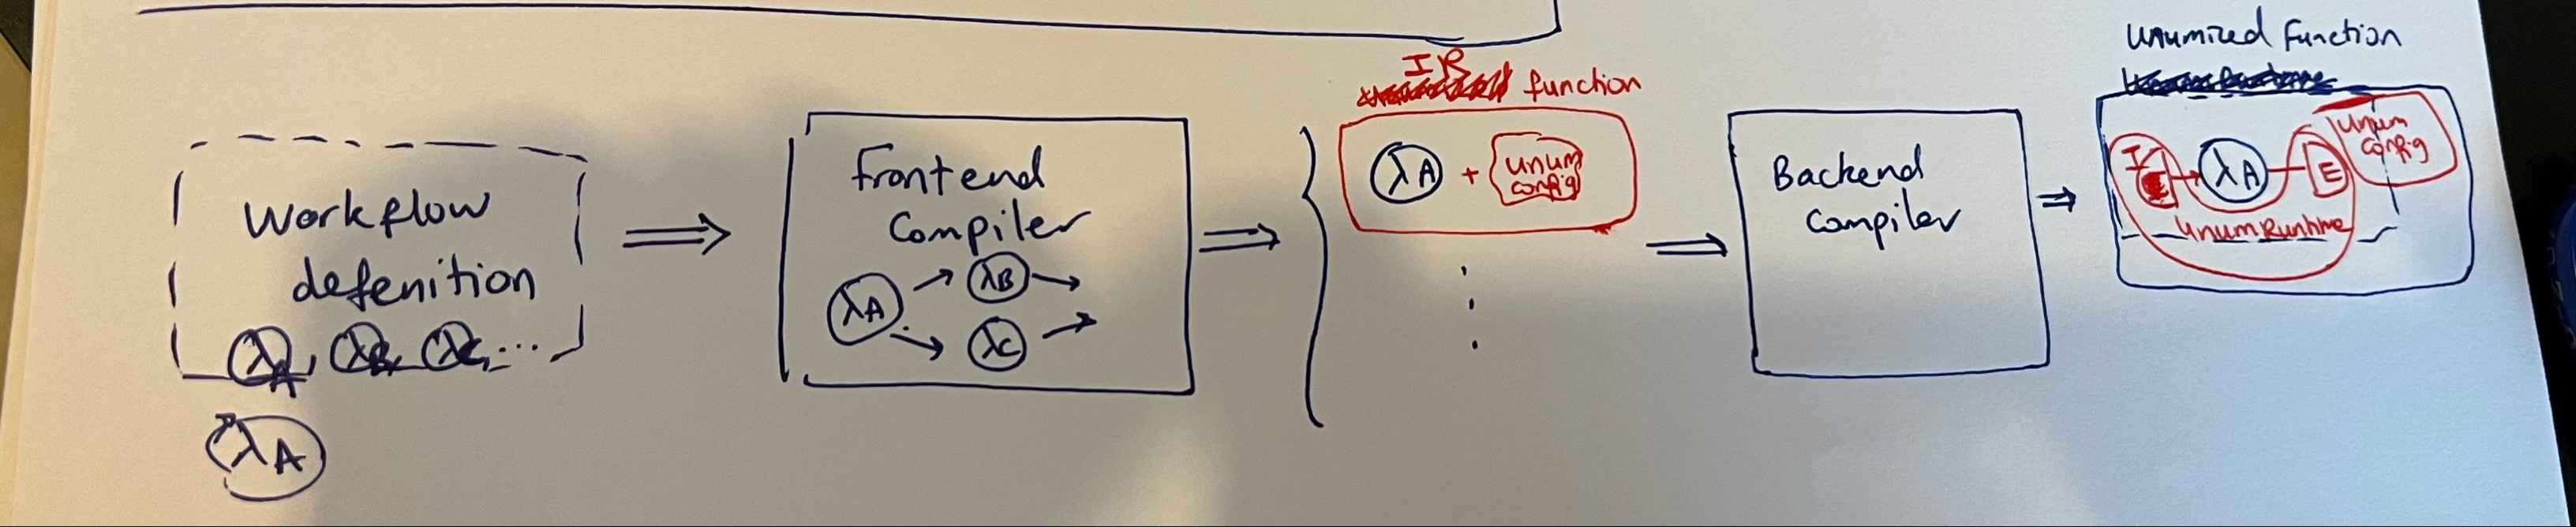
\includegraphics[width=\columnwidth]{figures/architecture.png}
        \caption{Stateful serverless computations form a directed graph. Nodes
                are user defined FaaS functions and workflow ``gadgets'' that dictate the
                communication pattern between user functions.}
        \label{fig:arch:unum-compile-time}
        % unum injects gadgets to functions at compile time. But more
        % specifically, unum injects an encoding of gadgets at compile time.
        % The encoding expresses control-flow transitions just like what the
        % high-level workflow definition.
    \end{subfigure}
    \begin{subfigure}[b]{\columnwidth}
    \centering
        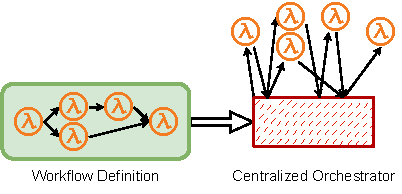
\includegraphics[width=0.8\columnwidth]{figures/unum-arch-centralized.pdf}
        \caption{A typical stateful serverless system drives workflow logic
                 using a centralized controller that manages the computation's state-machine.}
        \label{fig:arch:centralized}
    \end{subfigure}
    \hfill
    \begin{subfigure}[b]{\columnwidth}
    \centering
        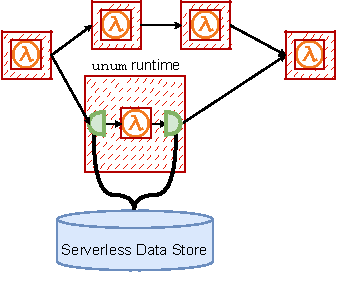
\includegraphics[width=0.5\columnwidth]{figures/unum-arch-runtime.pdf}
        \caption{\name{} decentralizes controller logic by running local state
                 transitions alongside Faas functions inside the \name{} runtime
                library. There is no centralized controller, instead \name{} relies on existing
                serverless datastores such as DynamoDB or Cosmos DB.}
        \label{fig:arch:unum-runtime}
    \end{subfigure}
    \caption{\name{} System Overview. Serverless computations form a directed
            graph that encode sequential and data dependencies between functions. Workflow
            orchestrators drive these graphs by centralizing control flow logic and
            interposing on all communication between functions. \name{},
            instead, decentralizes control flow logic among the functions with
            no need for a separate orchestration system.}
    \label{fig:arch}
\end{figure*}


Similar to other workflow systems~\cite{aws-step-functions, google-workflows,
	google-cloud-composer, gg-atc}, in \name{} users define their workflows using
a high-level description language that (directly or indirectly) expresses the
control-flow in the form of directed graphs  where nodes are serverless
functions and edges are control-flow transitions between functions. \name{'s} modular and extensible design supports integration with all commonly used high-level languages, e.g., Step functions representing workflows as state machines and Google
Workflows, Apache Airflow, Dask, representing workflows as DAGs\footnote{Our current implementation of \name{} is based on Step Functions.}.
%

Different from existing systems where a centralized orchestrator executes
the control-flow graph, \name{} partitions the control flow logic;  embeds the control flow alongside each individual function; and executes the functions in a distributed manner, with no centralized controller or additional services. Figure~\ref{fig:arch:unum-compile-time} shows the steps involved. First, the  \name{} compiler transforms the high-level workflow into a directed graph representation, e.g., converting the Step function state machines to a directed graph. Using this graph, the compiler outputs an platform agnostic intermediate representation (IR) represented as a set of IR functions, i.e, the user functions with the \name{} config embedded into it. the \name{} config includes the configuration on transition from the current function to the next function(s). Thus, instead of having a global view of the control-flow (in an orchestrator), the control-flow is distributed among functions such that each function just need to know where next to send the output. 

Next, the \name{} backend compiler converts the IR functions into \textit{unumized} functions, i.e., platform specific FaaS functions embedded with a \name{} runtime for that platform and the \name{} config. The user then deploys these unumized functions instead of its original functions. Upon execution, based on the \name config, the \name{} runtime  transparently, and in a decentralized manner, transitions data accordingly from one function to the next while also providing support for complex patterns such as fan-in. Additionally, the
runtime implements a checkpointing mechanism that ensures exactly-once
semantics (Section \shadi{?}).

This two step process in \name{} with the IR representation, enables portability to different function platforms (e.g., AWS Lambda or Azure Functions), and compatibility to different high-level languages as long as they can be compiled to a directed graph. Our current implementation is based on Step Functions as the API and AWS Lambda as the backend.



 


\dhl{TODO: Explain the purpose and use of the data store early on in the
	design portion of the paper. Probably also a good idea to motivate the use of
	data store in the background section.}





%During execution, the \name{} runtime performs control-flow transitions by
%running its assigned gadget (Figure~\ref{fig:arch:unum-runtime}). The runtime
%transparently interposes on user code entry and exit. On entry, the runtime
%reads data sent by the caller and passes it to user code. On exit, the runtime
%gets user code result and invokes the next function with it. Additionally, the
%runtime implements a checkpointing mechanism that ensures exactly-once
%semantics.
%
%\dhl{say more about exactly-once semantics here?}


\amit{TODO: gadgets are the secret sauce, in particular noticing that fan-in needs to
be split between the source and target functions \emph{and} that source
functions must coordinate.}
\amit{TODO: gadgets don't run where programmers express them. Example with
fan-in. This is kind of the ``magic'' of the front-end compiler.}
\dhl{I'm not sure the above 2 statements are true. Maybe because I didn't
understand your "move" gadgets mental model and it can work. Let's chat.}


%%%%%%%%%%%%%%%%%%


\subsection{\name{} Intermediate Representation}\label{sec:ir}
The \name{} compiler converts high-level workflow definitions into an intermediate representation (IR). The IR couples each user function with a platform agnostic \name{} config file containing the details on how to transition from that function to the next function(s). Specifically, the \name{} config includes: i. \textit{which} function(s) to call next, ii. \textit{when} to call the next function(s), iii. \textit{what} to send to the next function(s). 

\begin{table}[t!]
	\centering
	\begin{tabular}{ |m{8em}| m{13em} | }
		\hline
		\texttt{chain(a,b) }& Invokes function \texttt{b} with the output of \texttt{a} \\
		\hline
		\texttt{fanOut(a, [b])} & Invokes each element of \texttt{[b]} with the output from \texttt{a} \\
		\hline
		\texttt{map(a, b)} & Invokes \texttt{b} once for each element in the vector output of \texttt{a} \\
		\hline
		\texttt{fanIn([a], b)} & Invokes \texttt{b} once with the vector of outputs from each of \texttt{[a]} \\
		\hline
	\end{tabular}
	\caption{\name{} workflows express complex interactions using a small set of
		gadgets. \texttt{a} and \texttt{b} are names that identify specific function
		instances in the control flow graph.}
	\label{tab:gadgets}
\end{table}


As described in Table~\ref{tab:gadgets}, \name{} supports four general  control-flow patterns:
\begin{itemize}
	\item \textit{chain} connecting two functions. Chaining is a simple but common control-flow pattern, e.g.,  a function (source) processing sensor data followed by another function (destination) adjusting an
	actuator. 
	\item \textit{map} \shadi{??}
	\item \textit{fan out}  e.g.,  an social network application performing
	several independent functions given a new user post, such as URL shortening
	and resolving other users mentioned in the post. 
	\item \textit{fan in}. \shadi{@David: describe pattern in the text. also merge with descriptions in later section. move to here.} 
\end{itemize}
 These four patterns  can express a rich variety of workflows
efficiently, including a superset of workflows expressible in AWS Step
Functions and all workflows we encountered.  

In practice, the \name{} config of a particular transition pattern is  is a set of static configuration
files written in JSON. The compiler drives these files, but developers can also directly write these files. 
There should be one configuration file for each transition and it
is placed in the source function. During
execution, the \name{} runtime reads the file and performs control-flow
transitions to the next function(s) based on the configuration.


Figure~\ref{fig:arch2} shows examples for each transition type encoded
by the \name{}~IR. The \texttt{Name} field identifies the source function, which is also the function where the
configuration file is placed. The \texttt{Next} field identifies the function
to which the destination function(s) and the
\texttt{InputType} field helps define the transition type. The value
\texttt{Scalar} instructs the runtime to treat user function's output as a
single entity, and when the \texttt{Next} field contains only one object
(i.e., not an array), it represents a \texttt{chain} pattern; whereas when the
\texttt{Next} field is an array, it represents a \texttt{fanOut} pattern.
\texttt{map} pattern have a special \texttt{Map} value for the
\texttt{InputType} field as it instructs the runtime to expect and treat the
output of the user function as an iterable. \shadi{add sentence on fan-in}.



\shadi{talk about dynamic runtime behavior and how that is encoded somewhere.}
%The goal of the \name{}~IR is to not only identify which transition pattern the
%runtime should execute (Figure\shadi{?}) but also contain enough information so that the \name{}
%runtime knows what to do when encountering dynamic runtime behavior,


%\dhl{We give an overview of how the \name{} IR language works in this section, but
%	the full language features and design rationales are beyond the scope of this
%	paper.}



\begin{figure*}[t!]
	\centering
	\begin{subfigure}[t]{\columnwidth}
		\centering
		\begin{minted}[
			frame=single,
			fontsize=\footnotesize
			]{json}
			{
				"Name": "F",
				"Next": {
					"Name": "G",
					"InputType": "Scalar"
				}
			}
		\end{minted}
		\caption{\texttt{chain} pattern that invokes function \texttt{G} with
			\texttt{F}'s result}
		\label{fig:gadget-examples-chain}
	\end{subfigure}
	\begin{subfigure}[t]{\columnwidth}
		\centering
		\begin{minted}[
			frame=single,
			fontsize=\footnotesize
			]{json}
			{
				"Name": "F",
				"Next": {
					"Name": "G",
					"InputType": "Map"
				}
			}
		\end{minted}
		\caption{\texttt{map} pattern that invokes a parallel instance of
			\texttt{G} for each element of the vector output of \texttt{F}}
		\label{fig:gadget-examples-map}
	\end{subfigure}
	\hfill
	\begin{subfigure}[t]{\columnwidth}
		\centering
		\begin{minted}[
			frame=single,
			fontsize=\footnotesize
			]{json}
			{
				"Name": "F",
				"Next": [
				{
					"Name": "G",
					"InputType": "Scalar"
				},
				{
					"Name": "H",
					"InputType": "Scalar"
				}
				]
			}
		\end{minted}
		\caption{\texttt{fanOut} pattern that invokes function \texttt{G} and
			\texttt{H} with the result of \texttt{F}}
		\label{fig:gadget-examples-fanout}
	\end{subfigure}
	\begin{subfigure}[t]{\columnwidth}
		\centering
		\begin{minted}[
			frame=single,
			fontsize=\footnotesize
			]{json}
			{
				"Name": "F",
				"Next": {
					"Name": "G",
					"InputType": {
						"Fan-in": {
							"Values": [
							"F-unumIndex-*"
							]
						}
					}
				}
			}
		\end{minted}
		\caption{\texttt{fanIn} pattern that invokes function \texttt{G} with
			the result of all \texttt{F} instances of a \texttt{map}.}
		\label{fig:gadget-examples-fanin}
	\end{subfigure}
	\caption{\name{} System Overview. Serverless computations form a directed
		graph that encode sequential and data dependencies between functions. Workflow
		orchestrators drive these graphs by centralizing control flow logic and
		interposing on all communication between functions. \name{},
		instead, decentralizes control flow logic among the functions with
		no need for a separate orchestration system.}
	\label{fig:arch2}
\end{figure*}



%%%%%%%%%%%%%%%%%%%%%

%\section{Gadgets}\label{sec:gadgets}


\subsection{\name{'s} transition patterns  \shadi{suggested names?}}


A key challenge in decentralizing control-flow is determining where to store
control-flow state and how to execute transitions, without a global view of the orchestrator. 
Logically, each pattern is designed as
a pair of nodes: an ingress node and an egress node. The egress node is appended to the
upstream function and the matching ingress node is prepended to the immediate
downstream function(s).
Every user function in
\name{} has exactly one input edge coming from an ingress node and one output
edge going to an egress node, i.e., the user function is invoked once with a
single value by an ingress node and outputs its result to a single egress
node. 

The \name{} backend compiler converts the IR representation of functions  to platform specific \name{} runtimes with pairs of ingress/egress nodes (Figure \shadi{??}). The runtime then, based on the transition patterns embeded in \name{} config file, executes the patterns accordingly in each egress/ingress point. In this section we describe what exact execution logic does each pattern map to at the ingress and egress points. We note that \name{} runtime only uses the basic serverless abstractions, universally supported by current platforms, and are platform agnostic.
Specifically, it relies
on an asynchronous invocation API for FaaS functions and a strongly consistent
data store that supports conditional writes (for fan-in and exactly-once guarantees only). 

 \begin{figure}[t!]
 	\centering
 	\scalebox{.7}{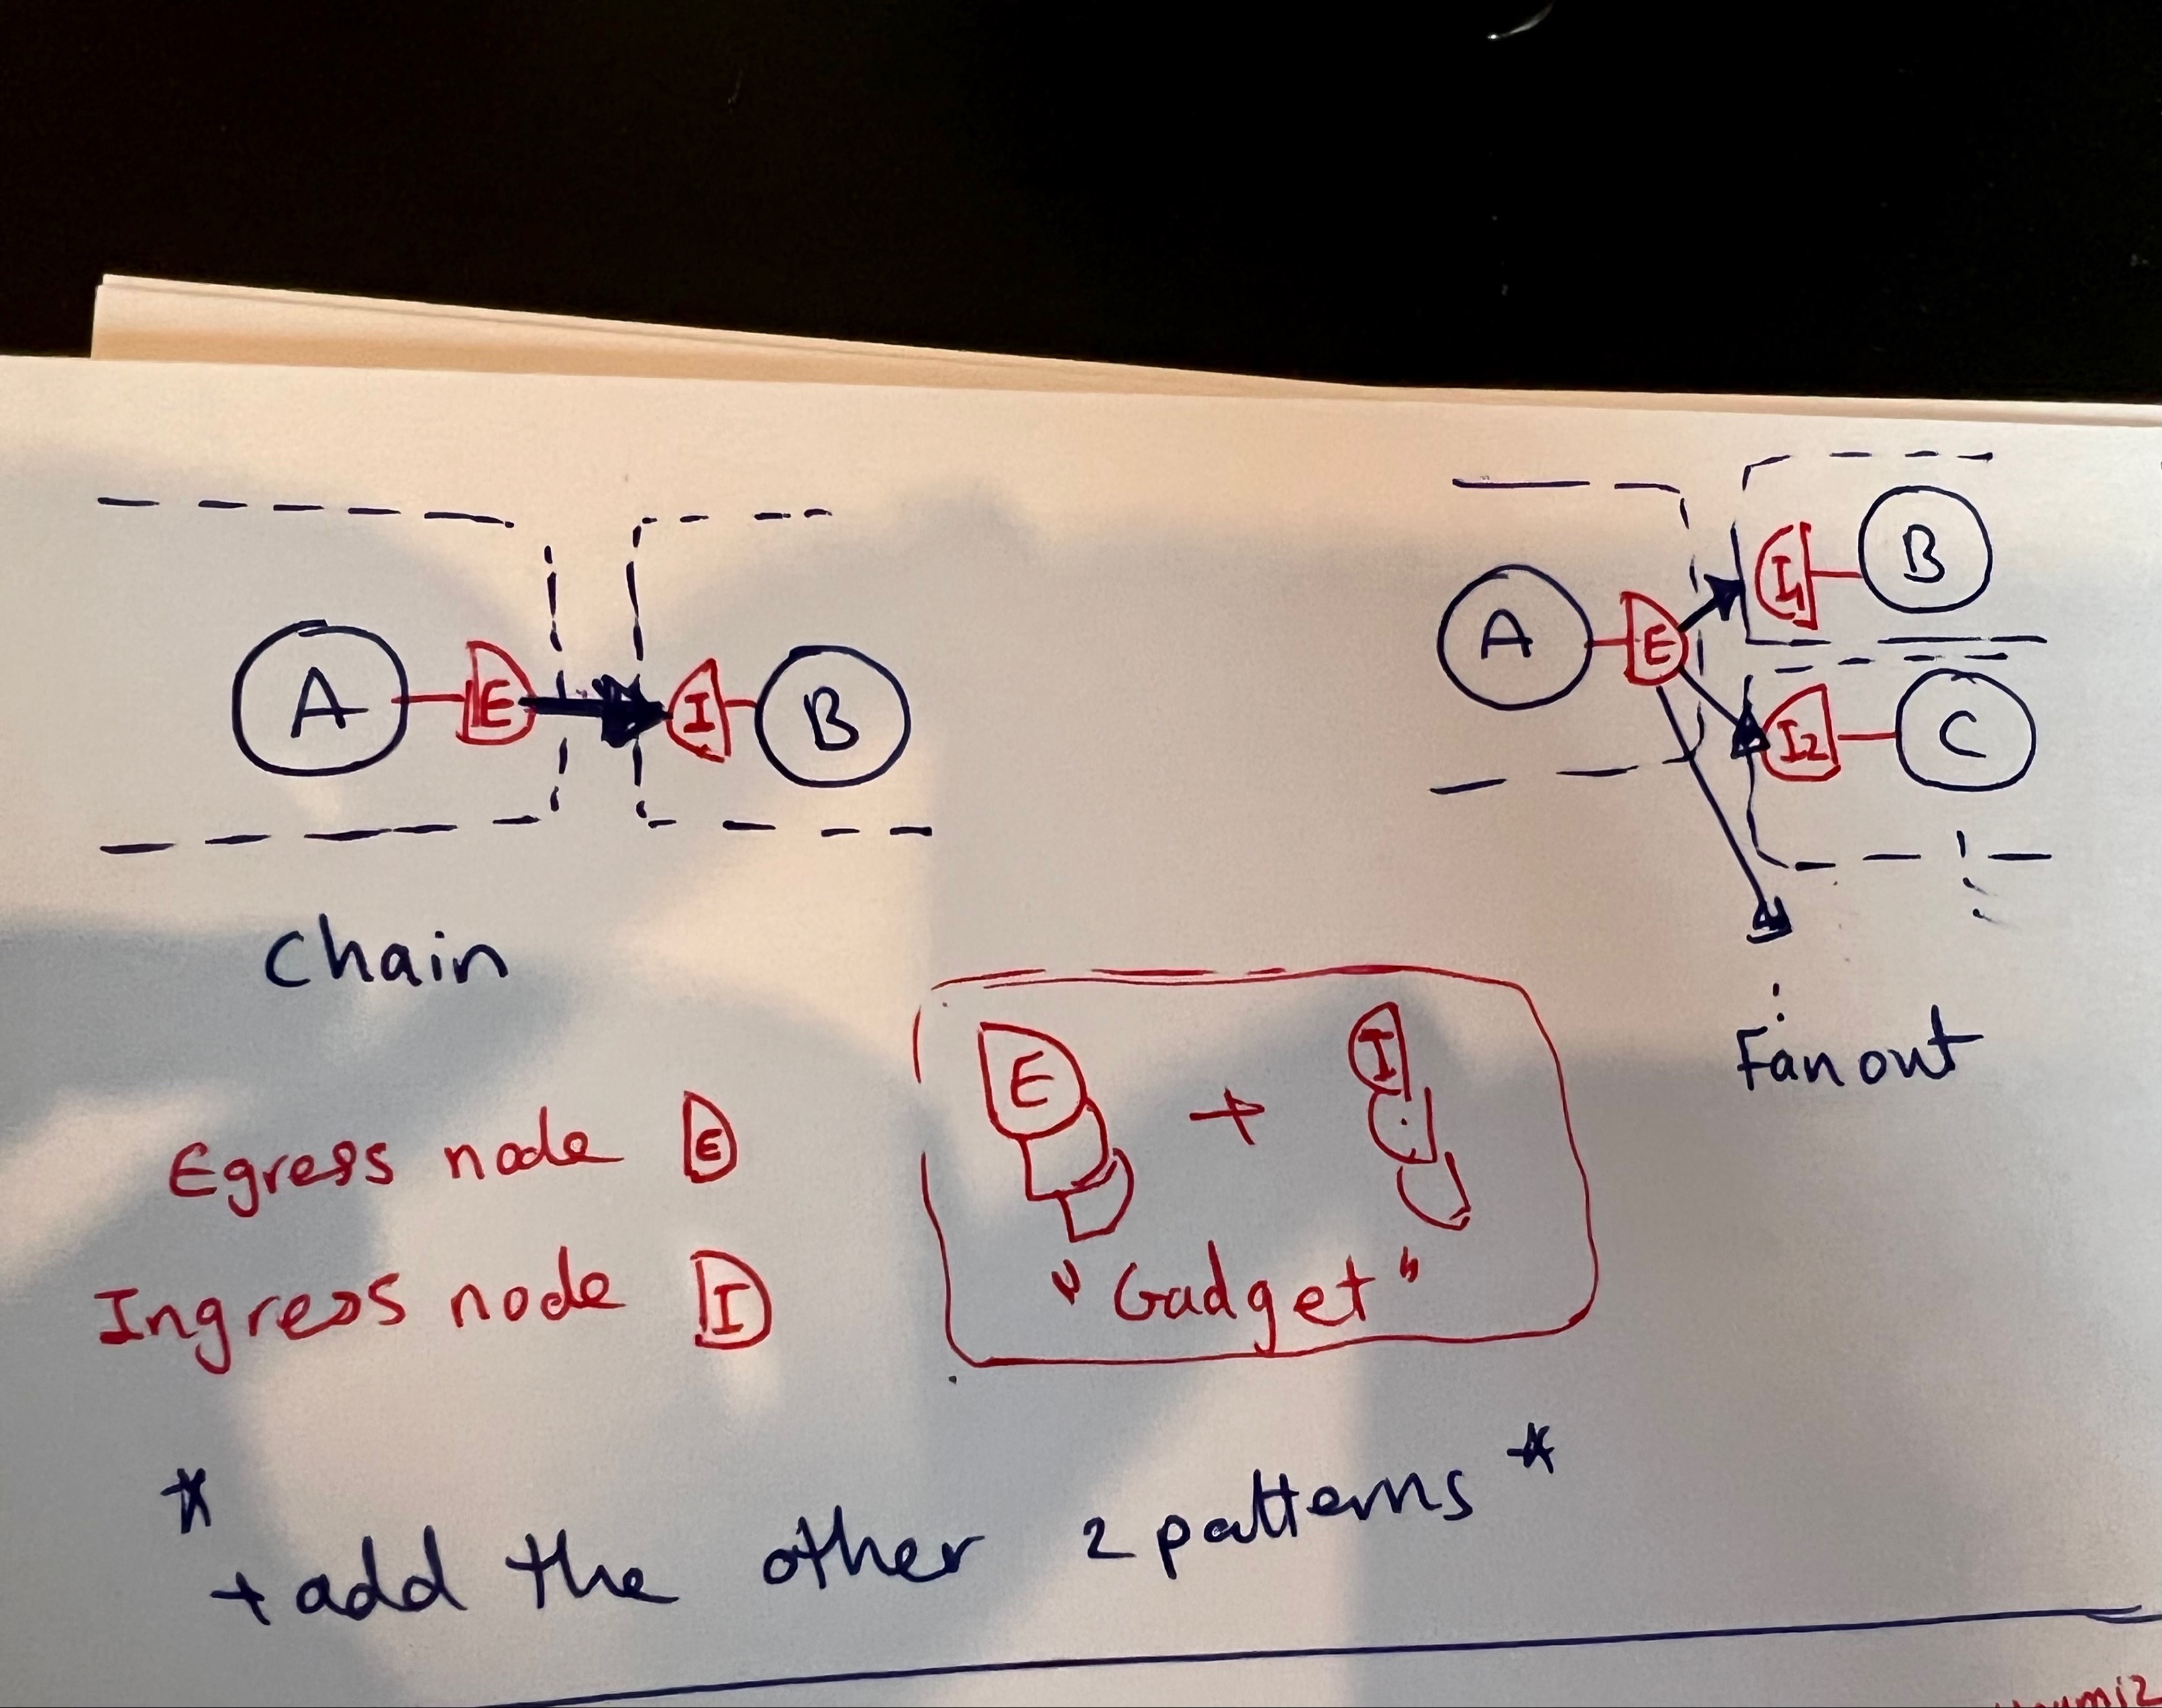
\includegraphics[width=\columnwidth]{figures/transitions.png}}
 	\caption{TODO}
 	\label{fig:transition}
 \end{figure}

\noindent\textbf{Chain}
The \texttt{chain} pattern connects two
user functions together by invoking the target with the result of the source.
As shown in Figure~\ref{fig:transition}, chaining consists of one egress node 
appended to the source function and one ingress is prepended to the target.
At runtime, the egress node gets the output of the source user function
and uses the platform's asynchronous function invocation API to call the
target function directly from the source. The ingress on the target reads the
data sent from source and passes it to the target user function. Depending on
the platform's implementation of asynchronous invoke API, the ingress might
read the input data from a data store or the received HTTP message.


\noindent\textbf{Fan-out}
The fan-out processes the output of a function in different
ways in parallel, by 
invoking vector of functions (branches) each with the output of the same
source function. The gadget consists of one egress node and many ingress
nodes (one per branch). Similar to chaining, the egress node runs with the
source function and it uses the asynchronous invocation API to invoke each
branch where each ingress node 
reads the input data sent from the source and passes it to its user function.

\shadi{:::::::::made changes only up to this point:::::::::::}


\dhl{"strongly consistent data store with conditional writes". Is this going
to raise eyebrows when we later mention S3? Because technically, S3 does not
have a conditional write API. We implement it with its object versions
feature, which has to be turned on when creating the bucket. Maybe better to
call it something else.}

% \dhl{I'm not sure it makes sense to treate fan-in specially on the directed
% graph level. In the previous version, the ingress gadget node on the fan-in
% doesn't really perform any \emph{control-flow logic}. It just reads the input
% data. And this is the same behavior across all gadgets. The ingress just read
% data, whether from a HTTP packet or from DynamoDB. You can pass a vector of
% pointers via a chain gadget and the ingress will do the same thing. But I
% guess more importantly, the ingress is simply and uniform enough that treating
% fan-in specially in our explanation doesn't add much value.}

\dhl{From previous version: "At compile-time, \name{} injects these gadgets
into the nearest function and executes them in the \name{} runtime that wraps
the function. Thus there is no system overhead for running the gadgets---they
are, effectively, embedded in the functions themselves."The last sentence is
unclear to me. Running gadgets incur latency and additional Lambda billing.}







\paragraph{Map}
An application may also perform the same function on multiple outputs of a
source function. For example, a photo management application might unpack an
archive of high-resolution images in one function and perform compression on
each of the resulting images. The \texttt{map} gadget invokes the same
function once for each element in a vector of outputs from the source
function. The algorithm and placement of \texttt{map} ingress and egress nodes
are identical to \texttt{fanOut}.

\dhl{TODO: talk about the dynamic aspect of Map}

\amit{TODO: Are there special considerations for exactly-once
semantics? i.e. is checkpointing different than it is in chaining?}
\dhl{No. In fact checkpoint works independently from the control-flow
patterns. The algorithm for exactly-once semantics is the same across all
gadgets.

Now specifically for fan-out it works like this: the fan-out initiator node
will checkpoint right after user code returns which saves the data that is
about to be fanned out. After checkpointing completes, the fan-out initiator
node invokes the branches. If it crashes at any point during the series of
invocations, unum retries the fan-out initiator lambda. The unum runtime on
the lambda will see that a checkpoint with its name already exists, and
therefore skips running the user function. But it will not skip retrying the
fan-out, and it restarts the fan-out \emph{from the beginning}, which will
result in duplicate instances for some or even all of the branches. But that
is OK. Because the unum runtime protects against duplicates and still ensures
exactly-once semantics. If the duplicates are concurrent (i.e., the original
branch instances are still running), we protects that with a conditional write
when checkpointing the results so only one instance of the duplicates will
win. If the duplicates are nonconcurrent (i.e., the original branch instances
already completed), the duplicates will skip running the user functions
altogether.

The fan-out initiator will keep retrying until a full fan-out is performed to
make sure at-least-once invocation.

% (explaining this makes me appreciate the consistency papers even more, 'cuz
% this stuff is hard to explain.)

So the patterns do not change the algorithms with which we provide exactly
once. They work independently from each other. The only real gotcha we need to
be careful with in \emph{implementing} exactly-once is nonidempotent
operations, as pointed out by you. Specifically, the synchronizations across
branches have to be idempotent. The purpose is prevent pre-mature fan-in.

Given the complexity of the exactly-once algorithm and the fact that it works
independently from gadgets, I think it works better if we have separate
section just for the execution guarantee and do not explain the details in
this section.}

\amit{TODO: I feel like there is a bunch of complexity, particularly with
fan-in, do with assigning indexes to branches, etc, that is part of the
platform-agnostic design of unum, so should be here. But I don't recall the
specifics. Are there also similar things for the other gadgets?}
\dhl{I'm not sure what you mean by "similar things". But the branch indexes
are assigned by the fan-\emph{out} node. The purpose is to give each node in
the graph a unique name. I really don't think we should discuss the naming
aspect in this section. I think this structure of writing the design works
very well if we keep the gadgets to be general algorithms for control-flow
patterns that are designed against an abstract serverless machine. We can talk
about what we require from the serverless abstraction, but we shouldn't talk
about the naming scheme. The gadget just cares that each function has a name,
that you can identify them. It does not care how. Then in the IR section, we
can talk about how the IR actually encodes the gadgets, and that's where we
can explain that (1). we need each function to have a unique name for fan-in
to work because we need to clearly identify which node's result to fan-in
from, and we can have multiple instances of the same function in the graph
because of fan-in and map. (2). our naming scheme is to assign an integer,
starting with 0 and incrementing monotonically by 1, to each branch. And
that's it. That's all the information we need at the IR level. And finally in
the runtime section, we show the input payload which has a field for the
branch index, and that's how we actually implement this piece of information.
And we explain that the fan-out node adds this field to the payload when
invoking each branch. It's like the storage layers where each layer adds a bit
more information to enable specific additional functionalities.}

\paragraph{Fan-in}

After processing data with many parallel branches, applications commonly want
to aggregate results. For example, a video encoder might divide a large video
into chunks, encode each in parallel and then concatenant all the encoded
chunks together. The \texttt{fanIn} gadget takes the outputs from a vector of
functions (the fan-in branches) and invokes a single ``sink'' function. The
\texttt{fanIn} gadget consists of one ingress node and many egress nodes. Each
fan-in branch is appended an egress node and the sink function is prepended
the only ingress node.

% TBD
%
% The \texttt{fanIn} gadget gadget ensures that the control-flow transition is
% \emph{wait-free} and that the sink function is invoked only once.
% Specifically, its semantics is that the sink function is invoked only once
% when all upstream functions in the vector have completed.

% To realize the semantics, the \texttt{fanIn} gadget has to solve several
% challenges. Access to branches data. wait-free. and synchronize.

The \texttt{fanIn} gadget ensures that the control-flow transition is
\emph{wait-free}. That is the sink function is invoked only when all upstream
functions in the vector have completed so that the sink function does have to
be spun up ahead of time and waste CPU cycles (and therefore extra billing)
idly waiting for upstream functions to finish. Moreover, the upstream
functions in \texttt{fanIn} simply terminates when done and do not wait for
each other either.

To achieve this, the \texttt{fanIn} egress always writes the output of its
user function to a data store. This serves two purposes: (1). it allows any of
the upstream functions to access the output of other upstream functions (2).
it signals the completion of a function. This way, each egress can simply
writes its output and terminate. Other egress nodes can still access completed
egress' data after they terminate. Any one of the egress can invoke the sink
function. And any one of the egress can see if other egress has completed or
not. \dhl{definitely needs better phrasing but hopeful the point makes sense}

Strongly consistent data store is important here because it prevents the
scenarios where all egress have written outputs but none of them sees that all
have completed, which results in the sink function never invoked.

Additionally, \texttt{fanIn} makes sure that when the sink function is
invoked, it is invoked only once. \name{} achieves this by having the egress
nodes synchronize with each other via the same data store such that only the
last-to-finish egress invokes the sink function. Synchronization is done with
atomic read-after-write over a single object. Specific implementation depends
on the data store and we discuss the details in \S\ref{sec:impl}. But all we
need is strong consistency with conditional writes.

The last-to-finish egress invokes the sink function with a vector of pointers
to each upstream function's stored output. The pointers are the in same order
as the vector of upstream function names. The ingress on the sink function
dereferences each point by reading from the data store and passes a vector of
output values to its user function.

\dhl{?TODO: Say more about synchronization? That it needs to be idempotent
because functions can crash and be retried.}

\dhl{?TODO: Fan-in is a critical control-flow pattern to support and distinguishes \name{}
from ad-hoc trigger-based composition.  Do we want to constrast here? and what
should we say? Different from ad-hoc compositions: 1. use of data store 2.
Control flow logic not only on the caller but also on the callee 3. standard,
off-the-shelf primitives that's not application specific that developers build
from scratch.}

\dhl{?TODO: Fan-in expresses data dependencies. More flexible/expressive than
Step Functions because SF only supports dependencies within a state. unum
fan-in can specify any function in the workflow.}


\dhl{TODO: Show that gadgets are composible. For example a map gadget followed
by a fanIn.}



\dhl{Propose name change for gadget -> nexus}

% chain = invoke, fan-out = a bunch of invoke, one for each continuation;
% Additionally, in the case of Map, one invoke for each element of the array
% (output of the user function).  fan-in .... well.... let's see. The semantics
% is: invoke the fan-in function once when all of its inputs are ready. In
% practice, it is each branch synchronize over the data store to see if all
% branches have completed. The last branch to complete calls invoke on the fan-in
% function, and pass it pointers to all branches results/checkpoints in the data
% store. The fan-in function first reads the branches' results, in order, via the
% pointers, then pass them as input to the user code.



\subsection{Naming Scheme}\label{sec:ir:naming}

A key design challenge of the \name{} IR is to support dynamic runtime
behavior with statically generated configurations. For instance, the number of
parallel branches in a \texttt{map} depends on the output of the egress node
and cannot be known at compile-time. 

For instance, a workflow that consists of a \texttt{map} gadget followed by a
\texttt{fanIn} gadget (e.g., a serverless video encoder that divides a large
video into chunks, encodes each chunk in parallel and fan-in to a concatenant
function at the end), the number of parallel branches depends on the output of
the \texttt{map} egress node and cannot be known at compile-time. Furthermore,
\texttt{map} creates multiple instances of the same function. \name{} needs to
uniquely identify each \emph{runtime} instance so that \texttt{fanIn} can
execute correctly (e.g., not miss an instance or counting the same instance
twice).

To solve this problem, \name{} defines a naming scheme for runtime instances
in the control-flow graph and exposes a set of programming constructs. First,
\name{} requires each user function to have a user-defined name. This is also
a common requirement for existing serverless systems when developers deploy
their functions. Next, each branch in a \texttt{map} and \texttt{fanOut}
gadget is assigned an integer index, starting from zero, and the $i^th$ branch
is named \texttt{<FunctionName>-unumIndex-\emph{i}}. For nested fan-outs, the
indexes are delimited with periods. For example,
\texttt{<FunctionName>-unumIndex-\emph{i.j}} identifies the $i^{th}$ branch in
the outer loop and $j^{th}$ in the inner loop.

To identify all branches, the \name{}~IR supports glob patterns, such as
\texttt{*}, when specifying runtime instances' names.
Figure~\ref{fig:gadget-examples-fanin} shows a \texttt{fanIn} example that
invokes \texttt{G} with the outputs from all instances of \texttt{F}.

\subsection{Programmable Constructs/APIs?}

\begin{figure}[]
    \begin{minted}[
frame=single,
fontsize=\footnotesize
]{json}
{
"Name": "F",
"Next": [
    {
        "Name": "G",
        "InputType": "Scalar",
        "Conditional": "$ret < 0"
    },
    {
        "Name": "H",
        "InputType": "Scalar",
        "Conditional": "$ret >= 0"
    }
]
}
    \end{minted}
    \caption{\texttt{F} branches on the user function's result by
    combining \texttt{fanOut} gadget with \texttt{Conditional}}
    \label{fig:gadget-examples-branch}
\end{figure}

In addition to the naming scheme, the IR also provides a set of constructs
that directly controls dynamic behavior. The complete set of programmable
constructs are beyond the scope of this paper, but we highlight one
API---\texttt{Conditional}--- in this section that \name{} uses to enable
branching. Figure~\ref{fig:gadget-examples-branch} shows an example of using
the \texttt{Conditional} field to control whether to run a gadget based on the
user function's output (\texttt{\$ret}). Combining \texttt{Conditional} with
\texttt{fanOut}, we can express branching logic in the control-flow. \dhl{can
also encode fold and for loops using Conditional to express the termination
condition.}

We highlight this example because it showcases the extensibility of \name{}'s
design: Given a small set of gadgets, \name{} can layer on top of them to
enable more dynamic control-flow logic.

\dhl{Platform-agnostic}

\section{Runtime}

\begin{figure}[]
    \begin{minted}[
    frame=single,
    fontsize=\footnotesize
  ]{json}
{
    "Data": {
        "Source": "http | dynamodb | s3 | ...",
        "Value": "<object> | [<pointers>]"
    },
    "Session": "uuid",
    "Fan-out": {
        "Index": "int",
        "Size": "int",
        "OuterLoop": {
            "Index": "int",
            "Size": "int"
        }
    }
}
    \end{minted}
    \caption{\name{} runtime input payload schema}
    \label{fig:input-format}
\end{figure}

The primary purpose of the \name{} runtime is to implement the gadgets with
platform-specific APIs and manage runtime metadata that is required by the
\name{} IR naming scheme and programmable constructs. We design the runtime to
wrap user code and transparently interpose on its entry and exit so that we do
not change how developers write application code.

 \name{} requires a specific input payload schema in JSON
(Figure~\ref{fig:input-format}). When a function is invoked, the input data is
first received by the runtime ingress. The ingress uses the \texttt{Data}
field to read the user function's input data. If the \texttt{Source} is
\texttt{http}, the input data is directly embedded in the \texttt{Value}
field. Otherwise, \name{} uses the pointers in \texttt{Value} to read the
input data from the intermediary data store.

After user function returns, the egress runtime gets its output and checks the
IR configuration to see if there is a gadget to execute. If no, it simply
terminates. If yes, it checks if the \texttt{Conditional} evaluates to true
and then executes the gadget egress.

\name{} keeps all runtime metadata in the input payload such that the
functions remain stateless and do not need to persist data via a data store
across invocations. \name{} uses the \texttt{Fan-out} field to store branch
indexes. The \texttt{Fan-out} field contains a recursive \texttt{OuterLoop}
field that \name{} uses to support nest fan-outs.

The runtime additionally uses a \texttt{Session} field to support concurrent
invocations of the same workflow. The \texttt{Session} field is a UUID string
that is unique to a workflow invocation and shared by all constituent function
instances in the invocation. Function checkpoint names are prefixed by the
\texttt{Session} string so that concurrently invocations do not overwrite each
other's data.

The \name{} runtime also implements exactly-once semantics with a
checkpointing mechanism which we discuss in the next section.


\section{Execution Guarantees}

Serverless systems only provide weak execution guarantees for functions.
Functions can crash for a variety of causes mid-execution. FaaS engines
usually only ensure at-least-once execution on individual functions. Invoking
a function once might result in duplicate instances that are potentially
concurrent.

\name{} provides exactly-once semantics for workflow execution despite the
challenges. Specifically, \name{} guarantees that even if there are
duplicates, whether they are concurrent or not, only one instance's result is
taken as the final result and propagates via gadgets to downstream nodes.
Other instances simply discard their results and terminate. Moreover, when a
workflow crashes mid-execution, \name{} does not retry from the beginning but
instead from the node of failure.

\name{} uses a checkpointing technique. After user code returns, the \name{}
runtime immediately creates a checkpoint file that contains the user code
results in the intermediary data store. The checkpoint is uniquely named with
the instance's name (i.e., the name according the
\name{}~IR's naming scheme (\S\ref{sec:ir:naming}), prefixed by the workflow
invocation's unique session ID) such that the existence of a checkpoint
implies the corresponding function has successfully completed its user
function. The create operation is a conditional write and only succeeds when
the file does not already exist. If there are concurrent duplicate instances,
only one of them will create the checkpoint. The others will receive an error
from the write operation and \name{} runtime will simply terminate the
instance. The instance that successfully creates a checkpoint will proceeds to
executing its gadget and propagate its result to downstream functions.

\dhl{TODO: Every time I mention "data store", I'm reminded of how little I've
talked about it so far. Need to fix.}

For nonconcurrent duplicates (e.g., retries), \name{} checks if a checkpoint
exists \emph{before} running its user code. If a checkpoint does not exist,
\name{} goes ahead and runs the user code. Otherwise, \name{} reads the data
from the checkpoint and use that as final result without running user code
again. Then \name{} will run the gadget to invoke the downstream function.
This is necessary because the duplicate might be a retry whose prior execution
crashed after checkpointing but before running the gadget. \name{} can
tolerate running a gadget more than once because of the same protection
against duplicates.

\name{} provides exactly-once semantics on the granularity of entire user
function, and therefore does not guarantee exactly-once for user code
operations that have external side effects.
